%------------------------------------------------------------------------------
%  DOCUMENT CONFIGURATION
%------------------------------------------------------------------------------

\documentclass[twoside, a4paper, titlepage]{article}

%------------------------------------------------------------------------------
%  PACKAGES
%------------------------------------------------------------------------------

\usepackage[utf8]{inputenc}
\usepackage[english]{babel}
\usepackage{csquotes} % Recommended

\usepackage[
  backend=biber,
  style=authoryear-ibid,
  maxcitenames=3,
  maxbibnames=100
]{biblatex}
\addbibresource{sources.bib}

\usepackage{fancyhdr} % Required for custom headers
\usepackage{lastpage} % Required to determine the last page for the footer
\usepackage{extramarks} % Required for headers and footers
\usepackage{graphicx} % Required to insert images
\usepackage{rotating} % Required for sideways figure
\usepackage{parskip} % Required for paragraph styling
\usepackage{float} % For having figures inline
\usepackage{amsmath}
\usepackage{amssymb}
\usepackage{hyperref} % For links
\usepackage{blindtext}
\usepackage{outlines}
\usepackage{tabularx}

\usepackage{tikz}
\restylefloat{figure}

%------------------------------------------------------------------------------

% Margins
\topmargin=-0.45in
\evensidemargin=0in
\oddsidemargin=0in
\textwidth=6.5in
\textheight=9.0in
\headsep=0.25in

% Numbering
% \setcounter{secnumdepth}{-1}

% Sans Serif Font
\renewcommand\rmdefault{cmss}

% Line spacing
\linespread{1.1}

% Images
\setlength\fboxsep{0pt}
\setlength\fboxrule{0.5pt}

\setlength\parskip{1.2em} % Space between paragraphs
\setlength\parindent{0pt} % Removes all indentation from paragraphs

%------------------------------------------------------------------------------
% TITLE PAGE
%------------------------------------------------------------------------------

\begin{document}

% Definition of blocks:
\tikzset{%
  block/.style    = {draw, thick, rectangle, minimum height = 3em,
    minimum width = 3em},
  sum/.style      = {draw, circle, node distance = 2cm}, % Adder
  input/.style    = {coordinate}, % Input
  output/.style   = {coordinate} % Output
}

\pagestyle{empty}

\newcommand{\reporttitle}{Blockchain-mediated Layered Access to Data}
\newcommand{\reportauthor}{Frederick Lindsey}
\newcommand{\reportsupervisor}{Dr. William Knottenbelt}
\newcommand{\reporttype}{BEng. Individual Project Report}

\begin{titlepage}

\newcommand{\HRule}{\rule{\linewidth}{0.5mm}}

\centering % Center remainder of the page
\vspace{1cm}


%-------------------------
%	HEADING SECTIONS
%-------------------------

\textsc{\LARGE \reporttype}\\[1.5cm]
\textsc{\Large Imperial College London}\\[0.5cm]
\textsc{\large Department of Computing}\\[0.5cm]

%--------------------------
%	TITLE SECTION
%--------------------------

\includegraphics[width = 4cm]{images/imperial_college_london_coat_of_arms}\\[0.5cm]

\HRule \\[0.4cm]
{ \huge \bfseries \reporttitle}\\
\HRule \\[1.5cm]

%--------------------------
%	AUTHOR SECTION
%--------------------------

\large
\begin{minipage}{0.5\textwidth}

\textit{Author:}\\
\reportauthor

\end{minipage}%
\begin{minipage}{0.5\textwidth}

\textit{Supervisor:}\\
\reportsupervisor

\end{minipage}

\vspace{7cm}
\makeatletter
\@date

\makeatother
\end{titlepage}


%------------------------------------------------------------------------------
% CONTENT
%------------------------------------------------------------------------------

% Identify key points including result of project
\abstract

Over the last several hundred years, the way we access and manage the world's data has radically changed. Recounting medieval times when there was little to no public record of a person's assets or information, this presents a stark comparison to today's society, where our data and identities are traded on a global market, often without our knowledge. This paper, and it's accompanying proof of concept, seeks to describe a method of reinstating the ownership of data that was once commonplace in previous centuries, without compromising on the free flowing and global nature of communication today.


% Acknowledge those who've technically or otherwise helped with completing the project
\renewcommand{\abstractname}{Acknowledgements}
\abstract

\thispagestyle{plain}
\pagenumbering{roman}
\setcounter{page}{2}

I'd like to thank Dr. William Knottenbelt and Dr. Robert Learney for their support and guidance through this project. Without their support this project would not have been a success.


% Set up the header and footer
\pagestyle{fancy}
\pagenumbering{arabic}
% \lhead{\docAuthorName} % Top left header
\rhead{\firstxmark} % Top right header
\lfoot{\lastxmark} % Bottom left footer
\cfoot{} % Bottom center footer
\rfoot{Page\ \thepage\ of\ \pageref{LastPage}} % Bottom right footer
\renewcommand\headrulewidth{0.4pt} % Size of the header rule
\renewcommand\footrulewidth{0.4pt} % Size of the footer rule

%------------------------------------------------------------------------------
% TABLE OF CONTENTS
%------------------------------------------------------------------------------

\tableofcontents

%------------------------------------------------------------------------------
% INTRODUCTION AND PREFACE
%------------------------------------------------------------------------------

% Write up understanding what the project is
\section{Introduction}

Over the last two hundred years, the way we access and manage the world's data has radically changed~\parencite{bankofengland:2016:online}.


%------------------------------------------------------------------------------
% BACKGROUND
%------------------------------------------------------------------------------

\section{Background}

% TODO: Swiss health identity card data

% - Privatisation of data
%   - Google, Facebook, NHS, Banks, retail stores (loyalty programs)
%   - Data Protection Act (limitations and corporate-focus)
% - User choice (who do I want to have my data and how)
% - Online identities
%   - Global identity tracking
%   - Conglomerate identity providers
% - Privatisation of data
%   - Google, Facebook, NHS, Banks, retail stores (loyalty programs)
%   - Data Protection Act (limitations and corporate-focus)
% - User choice (who do I want to have my data and how)
% - Online identities
%   - Global identity tracking
%   - Conglomerate identity providers
\subsection{Social Issues}

At the core of the motivation for this project lay several issues corresponding to the way in which society has been manipulated over time. It is my belief that we find ourselves in the current position without any ownership of our data because we've been keen (even greedy) as a society to reap the benefits of our data without considering the longer term security effects. We have dismissed the need to care and be responsible for our data. Below, I have highlighted the key domains in which we lack control that we should have over our personal data. Whilst written as a piece of fiction, we should be aware and concerned that ignoring the social issues with data transfer allows a world to form much similar to that of George Orwell's 1984~\autocite{orwell:1984:book} - we consider the likes of corporations synonymous with that of the 'Big Brother' character.

\subsubsection{Commoditisation of personal (and private) data}

There is no doubt that search tools such as those offered by Google and Microsoft, retail stores such as those offered by Amazon, and social networks such as Facebook and Twitter, dramatically enhance our lives and give us capabilities we would never have otherwise.

\subsubsection{Freedom to use personal data}



% - Introduction to PDLs
% - Relevance to project
% - Blockchain.info
% - Ethereum
% TODO: Any other relevant implementations
\subsection{Public De-centralised Ledgers}

\subsubsection{Introduction to Public De-centralised Ledgers}

\subsubsection{Relevance}

\subsubsection{Blockchain.info}

\subsubsection{Ethereum}

\subsubsection{IPFS}



% - Introduction to Proxy Re-Encryption
% - Relevance to project
% - ZeroDB
% TODO: Any other relevant implementations
\subsection{Proxy Re-Encryption}

\subsubsection{Introduction to Proxy Re-Encryption}

\blockquote{In a proxy re-encryption scheme a semi-trusted proxy converts a ciphertext for Alice into a ciphertext for Bob without seeing the underlying plaintext}\autocite{greenateniese:2006:article}

Fundamentally, proxy re-encryption is the process of taking a message $M_a$, encrypted by a party $P_a$, and re-encrypting it to be passed to party $P_b$. The message is then represented by $M_b$, such that it is only readable by party $P_b$. Through the re-encryption process, the message is never actually decrypted, such that the data is never revealed to any non-trusted parties (including the proxy itself). This process relies on the functional relationship between the two ciphertexts, with the characteristics of the proxy re-encryption processed determined by the topology of this function.

\begin{figure}[H]
  \centering
  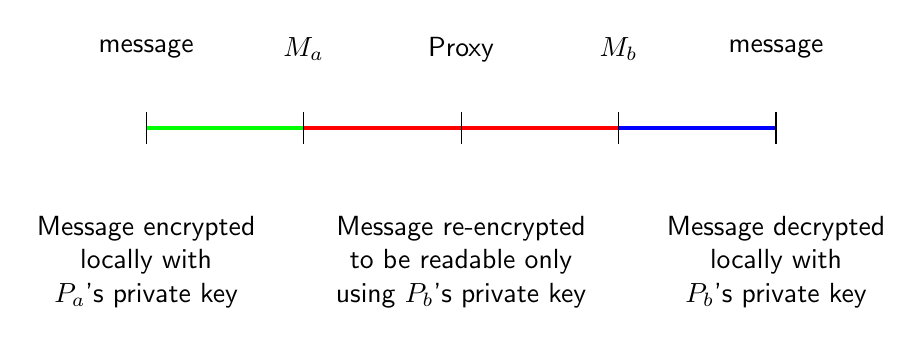
\begin{tikzpicture}

  \node at (0, 1)   {message} ;
  \node at (2, 1)   {$M_a$}   ;
  \node at (4, 1)   {Proxy}   ;
  \node at (6, 1)   {$M_b$}   ;
  \node at (8, 1)   {message} ;

  \draw [very thick, green] (0,0)   -- (2,0)   ;
  \draw [very thick, red]   (2,0)   -- (6,0)   ;
  \draw [very thick, blue]  (6,0)   -- (8,0)   ;
  \draw                     (0,-.2) -- (0, .2) ;
  \draw                     (2,-.2) -- (2, .2) ;
  \draw                     (4,-.2) -- (4, .2) ;
  \draw                     (6,-.2) -- (6, .2) ;
  \draw                     (8,-.2) -- (8, .2) ;

  \node[align=center, below] at (0, -1)%
    {Message encrypted\\locally with\\$P_a$'s private key};
  \node[align=center, below] at (4, -1)%
    {Message re-encrypted\\to be readable only\\using $P_b$'s private key};
  \node[align=center, below] at (8, -1)%
    {Message decrypted\\locally with\\$P_b$'s private key};

  \end{tikzpicture}
  \caption{
    Journey of a message using a proxy re-encryption scheme.
  }
\end{figure}


In figure \ref{fig:pre_example}, whether data is handled or manipulated by a fully trusted entity or not is indicated using green/blue and red lines respectively.

The encrypted message $M_a$ is passed to the semi-trusted proxy along with the re-encryption key (expressed as $f(E_a, e_b)$\footnote{$E_x$ represents the private key of a party $x$, $e_x$ represents the public key of a party $x$,})

% Delegation – allows a message recipient (keyholder) to generate a re-encryption key based on his secret key and the key of the delegated user. This re-encryption key is used by the proxy as input to the re-encryption function, which is executed by the proxy to translate ciphertexts to the delegated user's key. Asymmetric proxy re-encryption schemes come in bi-directional and uni-directional varieties.

% - In a bi-directional scheme, the re-encryption scheme is reversible—that is, the re-encryption key can be used to translate messages from Bob to Charlie, as well as from Charlie to Bob. This can have various security consequences, depending on the application. One notable characteristic of bi-directional schemes is that both the delegator and delegated party (e.g., Charlie and Bob) must combine their secret keys to produce the re-encryption key.
% - A uni-directional scheme is effectively one-way; messages can be re-encrypted from Bob to Charlie, but not the reverse. Uni-directional schemes can be constructed such that the delegated party need not reveal its secret key. For example, Bob could delegate to Charlie by combining his secret key with Charlie's public key.

% Transitivity – Transitive proxy re-encryption schemes allow for a ciphertext to be re-encrypted an unlimited number of times. For example, a ciphertext might be re-encrypted from Bob to Charlie, and then again from Charlie to David and so on. Non-transitive schemes allow for only one (or a limited number) of re-encryptions on a given ciphertext. Currently, there is no known uni-directional, transitive proxy re-encryption scheme. It is an open problem as to whether such constructions are possible.

\subsubsection{Applying Proxy Re-Encryption}



\subsubsection{ZeroDB}



% TODO: Research
% \section{Time-based Access For Encrypted Data}

TODO



% TODO: Research
% \input{sections/background/accessing_encrypted_object_fields}


% TODO: Research
% \input{sections/background/identity_storage}


%------------------------------------------------------------------------------
% POTENTIAL IMPLEMENTATION IDEAS
%------------------------------------------------------------------------------

\section{Implementation Considerations}

Since the core requirements of the project are architecture-independent to some degree, a simple solution which is not fully decentralised is a good option to begin with.

At current, a potential implementation utilises the following technologies:

\begin{outline}
  \1 AWS S3 (file/blob storage)
  \1 AWS EB (scalable application endpoints)
  \1 AWS RDS (SQL database)
  \1 Ethereum (Blockchain-based decentralised applications)
  \1 Electron (desktop application wrapper)
\end{outline}

Whilst centralised, Amazon Web Services (AWS) provides a solid and stable platform for the deployment of the application. Well-tested and production-ready software such as PostgreSQL, Amazon S3, and Amazon Elastic Beanstalk (running docker) not only provide a durable and dependable deployment solution, but also allow the development and production environments to be mirrored such that development need not take place online.

% PARTY A
% Private (unencrypted?) data
% Private key / Public key pair

% PARTY B
% Private (unencrypted?) data
% Private key / Public key pair

% PROXY
% Public keys for all users / institutions (verifies the identity of a party and allows re-encryption)
% Re-encryption keys for each API access (requires the 3rd party to read data)
% Encrypted data (using owner's private key - not readable by anyone else)

% No private keys nor unencrypted data is shared in the network
% Upon granting access, the user's device generates the re-encryption key locally (potentially multiple keys whereby the data is readable by anyone but the data is verified to be encrypted by a particular device??)
% This would require the use of proxy-reencryption such that any data uploaded by any device could be re-encrypted to be decrypted by any of the user's devices

% User passes private and encrypted data to proxy
% User sends the re-encryption key and access
% Access logs are encrypted with the user's public key as blobs on blockchain - only readable by the user themselves
% Who owns data - where do we store data that is written by party a but belongs to party b?

% What about if you used IPFS across public hardware - individuals etc. to create the world's biggest network of file storage stations, the mining being the storage of files, paid for by people using the network to store encrypted data. Filecoin?

The application would be distributed such that it could run on desktop operating systems (Mac and Linux (Debian) initially\footnote{Deployment of other packages may incur more overhead unnecessary at this point}). This means that the backend services of the project would be distinct from any front-end, whilst a public API offers the opportunity for third parties to contribute data and encourage user adoption.

The project architecture could be modelled, to some extent, by the following:

\begin{figure}[H]
  \centering
  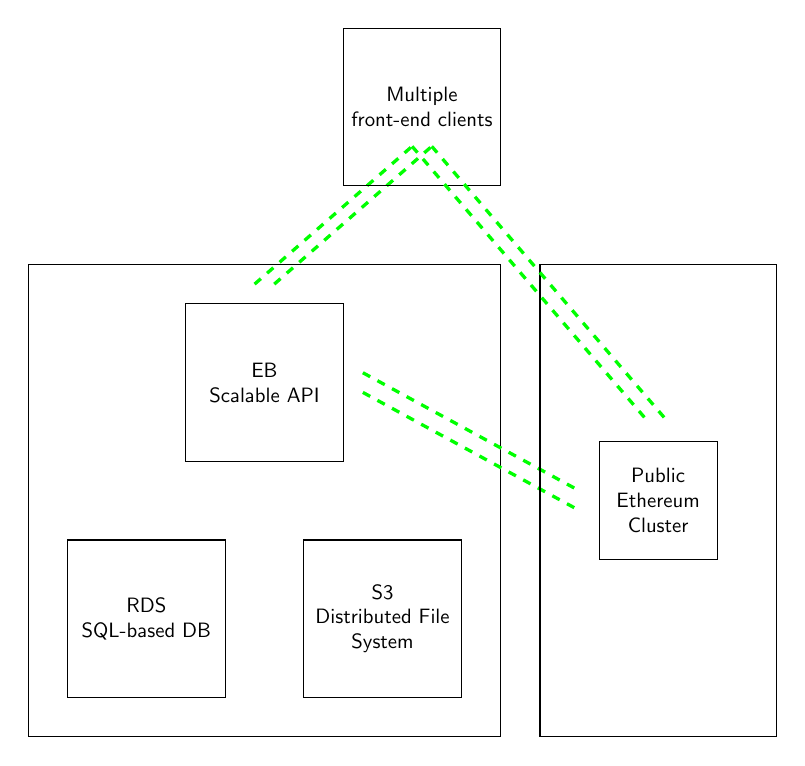
\begin{tikzpicture}[scale = 0.5, every node/.style={scale = 0.75}]

  % AWS Architecture
  \draw (-1, -1) rectangle (11, 11);
  \draw (0, 0) rectangle (4, 4);
  \draw (6, 0) rectangle (10, 4);
  \draw (3, 6) rectangle (7, 10);
  \draw[dashed, very thick, green] (4.75, 10.5) -- (8.75, 14);
  \draw[dashed, very thick, green] (5.25, 10.5) -- (9.25, 14);
  \draw[dashed, very thick, green] (7.5, 8.25) -- (13, 5.25);
  \draw[dashed, very thick, green] (7.5, 7.75) -- (13, 4.75);

  % Ethereum
  \draw (12, -1) rectangle (18, 11);
  \draw (13.5,  3.5) rectangle (16.5, 6.5);

  % Front-end services
  \draw (7, 13) rectangle (11, 17);
  \draw[dashed, very thick, green] (8.75, 14) -- (14.75, 7);
  \draw[dashed, very thick, green] (9.25, 14) -- (15.25, 7);

  \node[align=center] at (2, 2) { RDS\\SQL-based DB };
  \node[align=center] at (8, 2) { S3\\Distributed File\\System };
  \node[align=center] at (5, 8) { EB\\Scalable API };
  
  \node[align=center] at (9, 15) { Multiple\\front-end clients };
  
  \node[align=center] at (15, 5) { Public\\Ethereum\\Cluster };

  \end{tikzpicture}
  \caption{
    Potential architecture for proof of concept. Shows links between different systems using green, dashed lines. Each inner box referring to a specific service within a location (public or private). All links are made over public infrastructure.\textit{The Electron application that will be built as part of this proof of concept is assumed to be one of many front-end clients.}
  }
  \label{fig:arch_potential_1}
\end{figure}





%------------------------------------------------------------------------------
% PROJECT PLAN
%------------------------------------------------------------------------------

\section{Project Plan}

Over the course of the project, there will be several stages and for each of these stages an associated key milestone. Throughout this process, a mixture of research, discovery, implementation, and user testing must occur in order to give the project a well-rounded and well-evaluated outcome.

Below, I explain the desired timeline of the project and indicate when I intend to reach specific milestones.

\vspace{5 mm}
\begin{table}[!h]
  \centering
  \begin{tabularx}{0.9\textwidth}{ r | X }
    \textbf{10th February} & Complete Interim Report (Draft) \\
                           & At this point crucial research should have been undertaken to understand the viability of the project and to be able to assess it's preliminary chances of success. \\
                           [4ex]
    \textbf{17th February} & Prototype architecture \\
                           & Whilst working on preliminary architecture, the implementation of core features should have begun. By this point a more structured and well understood architecture should be written. \\
                           [4ex]
    \textbf{3rd March}     & Evaluate and consider second marker's comments
                           and advice \\
                           & After discussions with the second marker to the project, evaluate the points of concern and any advice on how to achieve the greatest success with the project. Move forward with this in mind and adjust any proposed plans or process as necessary. \\
                           [4ex]
    \textbf{5th March}     & First working prototype \\
                           & A basic working prototype must include the ability to read and write data at a basic level \\
                           [4ex]
    \textbf{7th May}       & Second working prototype \\
                           & A second working prototype should be made by this point. It must include basic desktop functionality and the ability to use multiple accounts to access 3rd party data (at different levels). \\
                           [4ex]
    \textbf{15th May}      & Project Health Checkup \\
                           & Given the length of time between here and the working prototype having been demonstrated to the supervisor in March, by this point some evaluation should be done in terms of reconsidering what the final goals are for the project in the remaining month. \\
                           [4ex]
    \textbf{19th June}     & Final Report Due \\
                           [4ex]
    \textbf{26th June}     & Submission of Project Archive
  \end{tabularx}
  \vspace{10 mm}
  \caption{
    Plan for project (given progress thus far)
  }
  \label{table:project_plan}
\end{table}


%------------------------------------------------------------------------------
% EVALUATION PLAN
%------------------------------------------------------------------------------

\section{Evaluation Plan}

% Evaluation plan (1-2 pages). Project evaluation is very important, so it's important to think now about how you plan to measure success. For example,

% - what functionality do you need to demonstrate?
% - What experiments to you need to undertake and what outcome(s) would constitute success?
% - What benchmarks should you use?
% - How has your project extended the state of the art?
% - How do you measure qualitative aspects, such as ease of use?

% These are the sort of questions that your project evaluation should address; this section should outline your plan.

\subsection{Demonstrable core functionality}

Below are lists of functionalities that are required for the project to have achieved success. In the case where the user is expected to be able to give multiple inputs in an either-or fashion, partial success is still achieved by implementing a subset of those inputs.

\subsubsection{Secure Distributed Storage}

\begin{outline}
  \1 Store encrypted data only, such that readable by the primary data owner only
  \1 Data input and output should never be decrypted - this should be provable
\end{outline}

\subsubsection{Secure Layered Access}

\begin{outline}
  \1 Allow the use of different access layers across a dataset
  \1 A party $P_a$ that is a member of a data-layer access group $D_b$, but may have extra (superceding) permissions will have access that is an extension of a party $P_b$ who is only a member $D_b$.
  \1 Disallow a party to see data exists if they do not have read access
\end{outline}

\subsubsection{Time-based Access}

\begin{outline}
  \1 Allow any user to request data from any other user who they can identify
  \1 Allow nominated 3rd parties to access data upon the successful granting of a request
  \1 Granted access to data is time-dependent using one of two inputs:
    \2 Set remaining time period
    \2 Set access termination date
\end{outline}

\subsubsection{Transparent and Public Logging}

\begin{outline}
  \1 For every access of a file (through the system), a record is written to a public ledger
  \1 All records of user access must be encrypted such that the primary data owner is the only party that can read them
  \1 The collapse of the system would not stop a user from viewing the logs for their data
  \1 The use of a public ledger does not cost the primary data owner anything
\end{outline}

\subsubsection{Secure Access and Access Management}

\begin{outline}
  \1 Unauthorised access to a user's account (maliciously or otherwise) does not allow reading a user's data
  \1 An actor must not be able to write to the access system such that they gain unauthorised access to data
\end{outline}

\subsection{Experimentation and Validation}

In order to verify that the above functionalities have been met, a series of experiments will need to be performed. These will include but are not limited to:

\begin{outline}
  \1 Create two users. Use the first to request data from the second (given a username or other identity parameter).
  \1 Simulate the use of a security hierachy and observe whether the system is able to handle this as one would expect.
  \1 Validate that data for which access has been granted is accessible with the correct access permissions (multiple tests required)
  \1 Validate that data for which access is given in a time-sensitive manner is no longer available once this time period expires
  \1 Attempt to write transactions to the ledger the application uses to gain access to the user data
  \1 Ensure that under single-user and multi-user loads, access is correctly implemented
  \1 Simulate a malicious attack on a user's account and attempt to retrieve their data. Record what user security information is required as a minimum to access any part of the user's secure data.
\end{outline}

\subsection{User testing and evaluation}

Qualitative user data will be assessed using the front-end of the application created for demonstration purposes. It is important that users who would currently access and update such systems do not feel pain in using the developed prototype. It is also important that the user experience is similar to that expected by potential users. It is my intention to use members of the college community of varying technical abilities and select members of the public who work in relevant industries to test the useability of the application and give feedback to improve the user experience.

I will attend the Wearable Technology Show\footnote{London, UK-based event taking place on 7-8 March 2017 \url{http://www.wearabletechnologyshow.net/home}} where I will try to get as much market data as possible on the viability and demand for such an application in the market place. This will be largely from wearable technology providers who, for the health care case study, would likely provide the infrastructure for data input from end users.

% User feedback is necessary
% Comprehensive user feedback
% Concrete evidence of success: quantitative


% During the ideation stage of the project, and as part of my research to determine the criteria that would need to be met to deem the project a success, I quickly determined that a case study (or multiple) would be vital to give the project context. Multiple markets have been considered, but two seemed particularly appropriate:
%
% \begin{outline}
%   \1 Healthcare data
%   \1 National Security data
% \end{outline}
%
% As one of the largest markets for private data shared by a public company, I agreed with my supervisor that a suitable case study would be to provide secure accessible storage to front digital health data in the UK.
%
% Further to agreeing this, I have received input from an industry specialist, Dr. Robert Learney\footnote{Dr. Learney is a Dyson scholar from the Department of Bioengineering, Imperial College London}, in the field of digital health data. We discussed the current situation of digital health data in the UK market, with particular reference to the National Health Service~\footnote{\url{http://www.nhs.uk/pages/home.aspx}} (NHS) and what would be a requirement of a proof of concept that would solve some of the many issues with the current distribution and storage of current health data.
%
% The core criteria that this project must adhere to are:
%
% \begin{outline}
%   \1 Secure distributed storage
%   \1 Time-based access
%   \1 Transparent, public logging
%   \1 Secure access and access management
% \end{outline}
%
% Below, I have applied the use-case to the above criteria to outline the most significant output criteria to determine the project's success.


%------------------------------------------------------------------------------
% BIBLIOGRAPHY AND APPENDICES
%------------------------------------------------------------------------------

% All sources used for research etc.
\section{Bibliography}
\printbibliography[heading=none]


% Appendix
\section{Appendix}

\listoffigures

\listoftables


%------------------------------------------------------------------------------

\end{document}
